\documentclass[11pt]{article}

    \usepackage[breakable]{tcolorbox}
    \usepackage{parskip} % Stop auto-indenting (to mimic markdown behaviour)
    

    % Basic figure setup, for now with no caption control since it's done
    % automatically by Pandoc (which extracts ![](path) syntax from Markdown).
    \usepackage{graphicx}
    % Keep aspect ratio if custom image width or height is specified
    \setkeys{Gin}{keepaspectratio}
    % Maintain compatibility with old templates. Remove in nbconvert 6.0
    \let\Oldincludegraphics\includegraphics
    % Ensure that by default, figures have no caption (until we provide a
    % proper Figure object with a Caption API and a way to capture that
    % in the conversion process - todo).
    \usepackage{caption}
    \DeclareCaptionFormat{nocaption}{}
    \captionsetup{format=nocaption,aboveskip=0pt,belowskip=0pt}

    \usepackage{float}
    \floatplacement{figure}{H} % forces figures to be placed at the correct location
    \usepackage{xcolor} % Allow colors to be defined
    \usepackage{enumerate} % Needed for markdown enumerations to work
    \usepackage{geometry} % Used to adjust the document margins
    \usepackage{amsmath} % Equations
    \usepackage{amssymb} % Equations
    \usepackage{textcomp} % defines textquotesingle
    % Hack from http://tex.stackexchange.com/a/47451/13684:
    \AtBeginDocument{%
        \def\PYZsq{\textquotesingle}% Upright quotes in Pygmentized code
    }
    \usepackage{upquote} % Upright quotes for verbatim code
    \usepackage{eurosym} % defines \euro

    \usepackage{iftex}
    \ifPDFTeX
        \usepackage[T1]{fontenc}
        \IfFileExists{alphabeta.sty}{
              \usepackage{alphabeta}
          }{
              \usepackage[mathletters]{ucs}
              \usepackage[utf8x]{inputenc}
          }
    \else
        \usepackage{fontspec}
        \usepackage{unicode-math}
    \fi

    \usepackage{fancyvrb} % verbatim replacement that allows latex
    \usepackage{grffile} % extends the file name processing of package graphics
                         % to support a larger range
    \makeatletter % fix for old versions of grffile with XeLaTeX
    \@ifpackagelater{grffile}{2019/11/01}
    {
      % Do nothing on new versions
    }
    {
      \def\Gread@@xetex#1{%
        \IfFileExists{"\Gin@base".bb}%
        {\Gread@eps{\Gin@base.bb}}%
        {\Gread@@xetex@aux#1}%
      }
    }
    \makeatother
    \usepackage[Export]{adjustbox} % Used to constrain images to a maximum size
    \adjustboxset{max size={0.9\linewidth}{0.9\paperheight}}

    % The hyperref package gives us a pdf with properly built
    % internal navigation ('pdf bookmarks' for the table of contents,
    % internal cross-reference links, web links for URLs, etc.)
    \usepackage{hyperref}
    % The default LaTeX title has an obnoxious amount of whitespace. By default,
    % titling removes some of it. It also provides customization options.
    \usepackage{titling}
    \usepackage{longtable} % longtable support required by pandoc >1.10
    \usepackage{booktabs}  % table support for pandoc > 1.12.2
    \usepackage{array}     % table support for pandoc >= 2.11.3
    \usepackage{calc}      % table minipage width calculation for pandoc >= 2.11.1
    \usepackage[inline]{enumitem} % IRkernel/repr support (it uses the enumerate* environment)
    \usepackage[normalem]{ulem} % ulem is needed to support strikethroughs (\sout)
                                % normalem makes italics be italics, not underlines
    \usepackage{soul}      % strikethrough (\st) support for pandoc >= 3.0.0
    \usepackage{mathrsfs}
    

    
    % Colors for the hyperref package
    \definecolor{urlcolor}{rgb}{0,.145,.698}
    \definecolor{linkcolor}{rgb}{.71,0.21,0.01}
    \definecolor{citecolor}{rgb}{.12,.54,.11}

    % ANSI colors
    \definecolor{ansi-black}{HTML}{3E424D}
    \definecolor{ansi-black-intense}{HTML}{282C36}
    \definecolor{ansi-red}{HTML}{E75C58}
    \definecolor{ansi-red-intense}{HTML}{B22B31}
    \definecolor{ansi-green}{HTML}{00A250}
    \definecolor{ansi-green-intense}{HTML}{007427}
    \definecolor{ansi-yellow}{HTML}{DDB62B}
    \definecolor{ansi-yellow-intense}{HTML}{B27D12}
    \definecolor{ansi-blue}{HTML}{208FFB}
    \definecolor{ansi-blue-intense}{HTML}{0065CA}
    \definecolor{ansi-magenta}{HTML}{D160C4}
    \definecolor{ansi-magenta-intense}{HTML}{A03196}
    \definecolor{ansi-cyan}{HTML}{60C6C8}
    \definecolor{ansi-cyan-intense}{HTML}{258F8F}
    \definecolor{ansi-white}{HTML}{C5C1B4}
    \definecolor{ansi-white-intense}{HTML}{A1A6B2}
    \definecolor{ansi-default-inverse-fg}{HTML}{FFFFFF}
    \definecolor{ansi-default-inverse-bg}{HTML}{000000}

    % common color for the border for error outputs.
    \definecolor{outerrorbackground}{HTML}{FFDFDF}

    % commands and environments needed by pandoc snippets
    % extracted from the output of `pandoc -s`
    \providecommand{\tightlist}{%
      \setlength{\itemsep}{0pt}\setlength{\parskip}{0pt}}
    \DefineVerbatimEnvironment{Highlighting}{Verbatim}{commandchars=\\\{\}}
    % Add ',fontsize=\small' for more characters per line
    \newenvironment{Shaded}{}{}
    \newcommand{\KeywordTok}[1]{\textcolor[rgb]{0.00,0.44,0.13}{\textbf{{#1}}}}
    \newcommand{\DataTypeTok}[1]{\textcolor[rgb]{0.56,0.13,0.00}{{#1}}}
    \newcommand{\DecValTok}[1]{\textcolor[rgb]{0.25,0.63,0.44}{{#1}}}
    \newcommand{\BaseNTok}[1]{\textcolor[rgb]{0.25,0.63,0.44}{{#1}}}
    \newcommand{\FloatTok}[1]{\textcolor[rgb]{0.25,0.63,0.44}{{#1}}}
    \newcommand{\CharTok}[1]{\textcolor[rgb]{0.25,0.44,0.63}{{#1}}}
    \newcommand{\StringTok}[1]{\textcolor[rgb]{0.25,0.44,0.63}{{#1}}}
    \newcommand{\CommentTok}[1]{\textcolor[rgb]{0.38,0.63,0.69}{\textit{{#1}}}}
    \newcommand{\OtherTok}[1]{\textcolor[rgb]{0.00,0.44,0.13}{{#1}}}
    \newcommand{\AlertTok}[1]{\textcolor[rgb]{1.00,0.00,0.00}{\textbf{{#1}}}}
    \newcommand{\FunctionTok}[1]{\textcolor[rgb]{0.02,0.16,0.49}{{#1}}}
    \newcommand{\RegionMarkerTok}[1]{{#1}}
    \newcommand{\ErrorTok}[1]{\textcolor[rgb]{1.00,0.00,0.00}{\textbf{{#1}}}}
    \newcommand{\NormalTok}[1]{{#1}}

    % Additional commands for more recent versions of Pandoc
    \newcommand{\ConstantTok}[1]{\textcolor[rgb]{0.53,0.00,0.00}{{#1}}}
    \newcommand{\SpecialCharTok}[1]{\textcolor[rgb]{0.25,0.44,0.63}{{#1}}}
    \newcommand{\VerbatimStringTok}[1]{\textcolor[rgb]{0.25,0.44,0.63}{{#1}}}
    \newcommand{\SpecialStringTok}[1]{\textcolor[rgb]{0.73,0.40,0.53}{{#1}}}
    \newcommand{\ImportTok}[1]{{#1}}
    \newcommand{\DocumentationTok}[1]{\textcolor[rgb]{0.73,0.13,0.13}{\textit{{#1}}}}
    \newcommand{\AnnotationTok}[1]{\textcolor[rgb]{0.38,0.63,0.69}{\textbf{\textit{{#1}}}}}
    \newcommand{\CommentVarTok}[1]{\textcolor[rgb]{0.38,0.63,0.69}{\textbf{\textit{{#1}}}}}
    \newcommand{\VariableTok}[1]{\textcolor[rgb]{0.10,0.09,0.49}{{#1}}}
    \newcommand{\ControlFlowTok}[1]{\textcolor[rgb]{0.00,0.44,0.13}{\textbf{{#1}}}}
    \newcommand{\OperatorTok}[1]{\textcolor[rgb]{0.40,0.40,0.40}{{#1}}}
    \newcommand{\BuiltInTok}[1]{{#1}}
    \newcommand{\ExtensionTok}[1]{{#1}}
    \newcommand{\PreprocessorTok}[1]{\textcolor[rgb]{0.74,0.48,0.00}{{#1}}}
    \newcommand{\AttributeTok}[1]{\textcolor[rgb]{0.49,0.56,0.16}{{#1}}}
    \newcommand{\InformationTok}[1]{\textcolor[rgb]{0.38,0.63,0.69}{\textbf{\textit{{#1}}}}}
    \newcommand{\WarningTok}[1]{\textcolor[rgb]{0.38,0.63,0.69}{\textbf{\textit{{#1}}}}}


    % Define a nice break command that doesn't care if a line doesn't already
    % exist.
    \def\br{\hspace*{\fill} \\* }
    % Math Jax compatibility definitions
    \def\gt{>}
    \def\lt{<}
    \let\Oldtex\TeX
    \let\Oldlatex\LaTeX
    \renewcommand{\TeX}{\textrm{\Oldtex}}
    \renewcommand{\LaTeX}{\textrm{\Oldlatex}}
    % Document parameters
    % Document title
    \title{index}
    
    
    
    
    
    
    
% Pygments definitions
\makeatletter
\def\PY@reset{\let\PY@it=\relax \let\PY@bf=\relax%
    \let\PY@ul=\relax \let\PY@tc=\relax%
    \let\PY@bc=\relax \let\PY@ff=\relax}
\def\PY@tok#1{\csname PY@tok@#1\endcsname}
\def\PY@toks#1+{\ifx\relax#1\empty\else%
    \PY@tok{#1}\expandafter\PY@toks\fi}
\def\PY@do#1{\PY@bc{\PY@tc{\PY@ul{%
    \PY@it{\PY@bf{\PY@ff{#1}}}}}}}
\def\PY#1#2{\PY@reset\PY@toks#1+\relax+\PY@do{#2}}

\@namedef{PY@tok@w}{\def\PY@tc##1{\textcolor[rgb]{0.73,0.73,0.73}{##1}}}
\@namedef{PY@tok@c}{\let\PY@it=\textit\def\PY@tc##1{\textcolor[rgb]{0.24,0.48,0.48}{##1}}}
\@namedef{PY@tok@cp}{\def\PY@tc##1{\textcolor[rgb]{0.61,0.40,0.00}{##1}}}
\@namedef{PY@tok@k}{\let\PY@bf=\textbf\def\PY@tc##1{\textcolor[rgb]{0.00,0.50,0.00}{##1}}}
\@namedef{PY@tok@kp}{\def\PY@tc##1{\textcolor[rgb]{0.00,0.50,0.00}{##1}}}
\@namedef{PY@tok@kt}{\def\PY@tc##1{\textcolor[rgb]{0.69,0.00,0.25}{##1}}}
\@namedef{PY@tok@o}{\def\PY@tc##1{\textcolor[rgb]{0.40,0.40,0.40}{##1}}}
\@namedef{PY@tok@ow}{\let\PY@bf=\textbf\def\PY@tc##1{\textcolor[rgb]{0.67,0.13,1.00}{##1}}}
\@namedef{PY@tok@nb}{\def\PY@tc##1{\textcolor[rgb]{0.00,0.50,0.00}{##1}}}
\@namedef{PY@tok@nf}{\def\PY@tc##1{\textcolor[rgb]{0.00,0.00,1.00}{##1}}}
\@namedef{PY@tok@nc}{\let\PY@bf=\textbf\def\PY@tc##1{\textcolor[rgb]{0.00,0.00,1.00}{##1}}}
\@namedef{PY@tok@nn}{\let\PY@bf=\textbf\def\PY@tc##1{\textcolor[rgb]{0.00,0.00,1.00}{##1}}}
\@namedef{PY@tok@ne}{\let\PY@bf=\textbf\def\PY@tc##1{\textcolor[rgb]{0.80,0.25,0.22}{##1}}}
\@namedef{PY@tok@nv}{\def\PY@tc##1{\textcolor[rgb]{0.10,0.09,0.49}{##1}}}
\@namedef{PY@tok@no}{\def\PY@tc##1{\textcolor[rgb]{0.53,0.00,0.00}{##1}}}
\@namedef{PY@tok@nl}{\def\PY@tc##1{\textcolor[rgb]{0.46,0.46,0.00}{##1}}}
\@namedef{PY@tok@ni}{\let\PY@bf=\textbf\def\PY@tc##1{\textcolor[rgb]{0.44,0.44,0.44}{##1}}}
\@namedef{PY@tok@na}{\def\PY@tc##1{\textcolor[rgb]{0.41,0.47,0.13}{##1}}}
\@namedef{PY@tok@nt}{\let\PY@bf=\textbf\def\PY@tc##1{\textcolor[rgb]{0.00,0.50,0.00}{##1}}}
\@namedef{PY@tok@nd}{\def\PY@tc##1{\textcolor[rgb]{0.67,0.13,1.00}{##1}}}
\@namedef{PY@tok@s}{\def\PY@tc##1{\textcolor[rgb]{0.73,0.13,0.13}{##1}}}
\@namedef{PY@tok@sd}{\let\PY@it=\textit\def\PY@tc##1{\textcolor[rgb]{0.73,0.13,0.13}{##1}}}
\@namedef{PY@tok@si}{\let\PY@bf=\textbf\def\PY@tc##1{\textcolor[rgb]{0.64,0.35,0.47}{##1}}}
\@namedef{PY@tok@se}{\let\PY@bf=\textbf\def\PY@tc##1{\textcolor[rgb]{0.67,0.36,0.12}{##1}}}
\@namedef{PY@tok@sr}{\def\PY@tc##1{\textcolor[rgb]{0.64,0.35,0.47}{##1}}}
\@namedef{PY@tok@ss}{\def\PY@tc##1{\textcolor[rgb]{0.10,0.09,0.49}{##1}}}
\@namedef{PY@tok@sx}{\def\PY@tc##1{\textcolor[rgb]{0.00,0.50,0.00}{##1}}}
\@namedef{PY@tok@m}{\def\PY@tc##1{\textcolor[rgb]{0.40,0.40,0.40}{##1}}}
\@namedef{PY@tok@gh}{\let\PY@bf=\textbf\def\PY@tc##1{\textcolor[rgb]{0.00,0.00,0.50}{##1}}}
\@namedef{PY@tok@gu}{\let\PY@bf=\textbf\def\PY@tc##1{\textcolor[rgb]{0.50,0.00,0.50}{##1}}}
\@namedef{PY@tok@gd}{\def\PY@tc##1{\textcolor[rgb]{0.63,0.00,0.00}{##1}}}
\@namedef{PY@tok@gi}{\def\PY@tc##1{\textcolor[rgb]{0.00,0.52,0.00}{##1}}}
\@namedef{PY@tok@gr}{\def\PY@tc##1{\textcolor[rgb]{0.89,0.00,0.00}{##1}}}
\@namedef{PY@tok@ge}{\let\PY@it=\textit}
\@namedef{PY@tok@gs}{\let\PY@bf=\textbf}
\@namedef{PY@tok@gp}{\let\PY@bf=\textbf\def\PY@tc##1{\textcolor[rgb]{0.00,0.00,0.50}{##1}}}
\@namedef{PY@tok@go}{\def\PY@tc##1{\textcolor[rgb]{0.44,0.44,0.44}{##1}}}
\@namedef{PY@tok@gt}{\def\PY@tc##1{\textcolor[rgb]{0.00,0.27,0.87}{##1}}}
\@namedef{PY@tok@err}{\def\PY@bc##1{{\setlength{\fboxsep}{\string -\fboxrule}\fcolorbox[rgb]{1.00,0.00,0.00}{1,1,1}{\strut ##1}}}}
\@namedef{PY@tok@kc}{\let\PY@bf=\textbf\def\PY@tc##1{\textcolor[rgb]{0.00,0.50,0.00}{##1}}}
\@namedef{PY@tok@kd}{\let\PY@bf=\textbf\def\PY@tc##1{\textcolor[rgb]{0.00,0.50,0.00}{##1}}}
\@namedef{PY@tok@kn}{\let\PY@bf=\textbf\def\PY@tc##1{\textcolor[rgb]{0.00,0.50,0.00}{##1}}}
\@namedef{PY@tok@kr}{\let\PY@bf=\textbf\def\PY@tc##1{\textcolor[rgb]{0.00,0.50,0.00}{##1}}}
\@namedef{PY@tok@bp}{\def\PY@tc##1{\textcolor[rgb]{0.00,0.50,0.00}{##1}}}
\@namedef{PY@tok@fm}{\def\PY@tc##1{\textcolor[rgb]{0.00,0.00,1.00}{##1}}}
\@namedef{PY@tok@vc}{\def\PY@tc##1{\textcolor[rgb]{0.10,0.09,0.49}{##1}}}
\@namedef{PY@tok@vg}{\def\PY@tc##1{\textcolor[rgb]{0.10,0.09,0.49}{##1}}}
\@namedef{PY@tok@vi}{\def\PY@tc##1{\textcolor[rgb]{0.10,0.09,0.49}{##1}}}
\@namedef{PY@tok@vm}{\def\PY@tc##1{\textcolor[rgb]{0.10,0.09,0.49}{##1}}}
\@namedef{PY@tok@sa}{\def\PY@tc##1{\textcolor[rgb]{0.73,0.13,0.13}{##1}}}
\@namedef{PY@tok@sb}{\def\PY@tc##1{\textcolor[rgb]{0.73,0.13,0.13}{##1}}}
\@namedef{PY@tok@sc}{\def\PY@tc##1{\textcolor[rgb]{0.73,0.13,0.13}{##1}}}
\@namedef{PY@tok@dl}{\def\PY@tc##1{\textcolor[rgb]{0.73,0.13,0.13}{##1}}}
\@namedef{PY@tok@s2}{\def\PY@tc##1{\textcolor[rgb]{0.73,0.13,0.13}{##1}}}
\@namedef{PY@tok@sh}{\def\PY@tc##1{\textcolor[rgb]{0.73,0.13,0.13}{##1}}}
\@namedef{PY@tok@s1}{\def\PY@tc##1{\textcolor[rgb]{0.73,0.13,0.13}{##1}}}
\@namedef{PY@tok@mb}{\def\PY@tc##1{\textcolor[rgb]{0.40,0.40,0.40}{##1}}}
\@namedef{PY@tok@mf}{\def\PY@tc##1{\textcolor[rgb]{0.40,0.40,0.40}{##1}}}
\@namedef{PY@tok@mh}{\def\PY@tc##1{\textcolor[rgb]{0.40,0.40,0.40}{##1}}}
\@namedef{PY@tok@mi}{\def\PY@tc##1{\textcolor[rgb]{0.40,0.40,0.40}{##1}}}
\@namedef{PY@tok@il}{\def\PY@tc##1{\textcolor[rgb]{0.40,0.40,0.40}{##1}}}
\@namedef{PY@tok@mo}{\def\PY@tc##1{\textcolor[rgb]{0.40,0.40,0.40}{##1}}}
\@namedef{PY@tok@ch}{\let\PY@it=\textit\def\PY@tc##1{\textcolor[rgb]{0.24,0.48,0.48}{##1}}}
\@namedef{PY@tok@cm}{\let\PY@it=\textit\def\PY@tc##1{\textcolor[rgb]{0.24,0.48,0.48}{##1}}}
\@namedef{PY@tok@cpf}{\let\PY@it=\textit\def\PY@tc##1{\textcolor[rgb]{0.24,0.48,0.48}{##1}}}
\@namedef{PY@tok@c1}{\let\PY@it=\textit\def\PY@tc##1{\textcolor[rgb]{0.24,0.48,0.48}{##1}}}
\@namedef{PY@tok@cs}{\let\PY@it=\textit\def\PY@tc##1{\textcolor[rgb]{0.24,0.48,0.48}{##1}}}

\def\PYZbs{\char`\\}
\def\PYZus{\char`\_}
\def\PYZob{\char`\{}
\def\PYZcb{\char`\}}
\def\PYZca{\char`\^}
\def\PYZam{\char`\&}
\def\PYZlt{\char`\<}
\def\PYZgt{\char`\>}
\def\PYZsh{\char`\#}
\def\PYZpc{\char`\%}
\def\PYZdl{\char`\$}
\def\PYZhy{\char`\-}
\def\PYZsq{\char`\'}
\def\PYZdq{\char`\"}
\def\PYZti{\char`\~}
% for compatibility with earlier versions
\def\PYZat{@}
\def\PYZlb{[}
\def\PYZrb{]}
\makeatother


    % For linebreaks inside Verbatim environment from package fancyvrb.
    \makeatletter
        \newbox\Wrappedcontinuationbox
        \newbox\Wrappedvisiblespacebox
        \newcommand*\Wrappedvisiblespace {\textcolor{red}{\textvisiblespace}}
        \newcommand*\Wrappedcontinuationsymbol {\textcolor{red}{\llap{\tiny$\m@th\hookrightarrow$}}}
        \newcommand*\Wrappedcontinuationindent {3ex }
        \newcommand*\Wrappedafterbreak {\kern\Wrappedcontinuationindent\copy\Wrappedcontinuationbox}
        % Take advantage of the already applied Pygments mark-up to insert
        % potential linebreaks for TeX processing.
        %        {, <, #, %, $, ' and ": go to next line.
        %        _, }, ^, &, >, - and ~: stay at end of broken line.
        % Use of \textquotesingle for straight quote.
        \newcommand*\Wrappedbreaksatspecials {%
            \def\PYGZus{\discretionary{\char`\_}{\Wrappedafterbreak}{\char`\_}}%
            \def\PYGZob{\discretionary{}{\Wrappedafterbreak\char`\{}{\char`\{}}%
            \def\PYGZcb{\discretionary{\char`\}}{\Wrappedafterbreak}{\char`\}}}%
            \def\PYGZca{\discretionary{\char`\^}{\Wrappedafterbreak}{\char`\^}}%
            \def\PYGZam{\discretionary{\char`\&}{\Wrappedafterbreak}{\char`\&}}%
            \def\PYGZlt{\discretionary{}{\Wrappedafterbreak\char`\<}{\char`\<}}%
            \def\PYGZgt{\discretionary{\char`\>}{\Wrappedafterbreak}{\char`\>}}%
            \def\PYGZsh{\discretionary{}{\Wrappedafterbreak\char`\#}{\char`\#}}%
            \def\PYGZpc{\discretionary{}{\Wrappedafterbreak\char`\%}{\char`\%}}%
            \def\PYGZdl{\discretionary{}{\Wrappedafterbreak\char`\$}{\char`\$}}%
            \def\PYGZhy{\discretionary{\char`\-}{\Wrappedafterbreak}{\char`\-}}%
            \def\PYGZsq{\discretionary{}{\Wrappedafterbreak\textquotesingle}{\textquotesingle}}%
            \def\PYGZdq{\discretionary{}{\Wrappedafterbreak\char`\"}{\char`\"}}%
            \def\PYGZti{\discretionary{\char`\~}{\Wrappedafterbreak}{\char`\~}}%
        }
        % Some characters . , ; ? ! / are not pygmentized.
        % This macro makes them "active" and they will insert potential linebreaks
        \newcommand*\Wrappedbreaksatpunct {%
            \lccode`\~`\.\lowercase{\def~}{\discretionary{\hbox{\char`\.}}{\Wrappedafterbreak}{\hbox{\char`\.}}}%
            \lccode`\~`\,\lowercase{\def~}{\discretionary{\hbox{\char`\,}}{\Wrappedafterbreak}{\hbox{\char`\,}}}%
            \lccode`\~`\;\lowercase{\def~}{\discretionary{\hbox{\char`\;}}{\Wrappedafterbreak}{\hbox{\char`\;}}}%
            \lccode`\~`\:\lowercase{\def~}{\discretionary{\hbox{\char`\:}}{\Wrappedafterbreak}{\hbox{\char`\:}}}%
            \lccode`\~`\?\lowercase{\def~}{\discretionary{\hbox{\char`\?}}{\Wrappedafterbreak}{\hbox{\char`\?}}}%
            \lccode`\~`\!\lowercase{\def~}{\discretionary{\hbox{\char`\!}}{\Wrappedafterbreak}{\hbox{\char`\!}}}%
            \lccode`\~`\/\lowercase{\def~}{\discretionary{\hbox{\char`\/}}{\Wrappedafterbreak}{\hbox{\char`\/}}}%
            \catcode`\.\active
            \catcode`\,\active
            \catcode`\;\active
            \catcode`\:\active
            \catcode`\?\active
            \catcode`\!\active
            \catcode`\/\active
            \lccode`\~`\~
        }
    \makeatother

    \let\OriginalVerbatim=\Verbatim
    \makeatletter
    \renewcommand{\Verbatim}[1][1]{%
        %\parskip\z@skip
        \sbox\Wrappedcontinuationbox {\Wrappedcontinuationsymbol}%
        \sbox\Wrappedvisiblespacebox {\FV@SetupFont\Wrappedvisiblespace}%
        \def\FancyVerbFormatLine ##1{\hsize\linewidth
            \vtop{\raggedright\hyphenpenalty\z@\exhyphenpenalty\z@
                \doublehyphendemerits\z@\finalhyphendemerits\z@
                \strut ##1\strut}%
        }%
        % If the linebreak is at a space, the latter will be displayed as visible
        % space at end of first line, and a continuation symbol starts next line.
        % Stretch/shrink are however usually zero for typewriter font.
        \def\FV@Space {%
            \nobreak\hskip\z@ plus\fontdimen3\font minus\fontdimen4\font
            \discretionary{\copy\Wrappedvisiblespacebox}{\Wrappedafterbreak}
            {\kern\fontdimen2\font}%
        }%

        % Allow breaks at special characters using \PYG... macros.
        \Wrappedbreaksatspecials
        % Breaks at punctuation characters . , ; ? ! and / need catcode=\active
        \OriginalVerbatim[#1,codes*=\Wrappedbreaksatpunct]%
    }
    \makeatother

    % Exact colors from NB
    \definecolor{incolor}{HTML}{303F9F}
    \definecolor{outcolor}{HTML}{D84315}
    \definecolor{cellborder}{HTML}{CFCFCF}
    \definecolor{cellbackground}{HTML}{F7F7F7}

    % prompt
    \makeatletter
    \newcommand{\boxspacing}{\kern\kvtcb@left@rule\kern\kvtcb@boxsep}
    \makeatother
    \newcommand{\prompt}[4]{
        {\ttfamily\llap{{\color{#2}[#3]:\hspace{3pt}#4}}\vspace{-\baselineskip}}
    }
    

    
    % Prevent overflowing lines due to hard-to-break entities
    \sloppy
    % Setup hyperref package
    \hypersetup{
      breaklinks=true,  % so long urls are correctly broken across lines
      colorlinks=true,
      urlcolor=urlcolor,
      linkcolor=linkcolor,
      citecolor=citecolor,
      }
    % Slightly bigger margins than the latex defaults
    
    \geometry{verbose,tmargin=1in,bmargin=1in,lmargin=1in,rmargin=1in}
    
    

\begin{document}
    
    \maketitle
    
    

    
    \renewcommand{\partname}{} % Réinitialiser partie

\textbf{Résumé~:} Ce livre vise à décrire une panoplie de méthodes de
traitement d'images satellites avec le langage Python. Celles et ceux
souhaitant migrer progressivement d'un autre logiciel d'imagerie et de
télédétection vers Python trouveront dans cet ouvrage les éléments pour
une transition en douceur. La philosophie de ce livre est de donner
toutes les clefs de compréhension et de mise en œuvre des méthodes
abordées dans Python. La présentation des méthodes est basée sur une
approche compréhensive et intuitive plutôt que mathématique, sans pour
autant négliger la rigueur mathématique ou statistique. Des rappels sur
les fondements en télédétection pourront apparaître au besoin afin
d'éclairer les approches techniques.

\textbf{Ce projet est en cours d'écriture et le contenu n'est pas
complet}


\includegraphics[width=0.5\textwidth,height=\textheight]{images/logos/under-construction-2408062_640.png}

\textbf{Remerciements~:} Ce manuel a été réalisé avec le soutien de la
fabriqueREL. Fondée en 2019, la fabriqueREL est portée par divers
établissements d'enseignement supérieur du Québec et agit en
collaboration avec les services de soutien pédagogique et les
bibliothèques. Son but est de faire des ressources éducatives libres
(REL) le matériel privilégié en enseignement supérieur au Québec.

\textbf{Maquette de la page couverture et identité graphique du livre~:}
.

\textbf{Mise en page~:} Samuel Foucher, Philippe Apparicio et
Marie-Hélène Gadbois Del Carpio.

\textbf{Révision linguistique~:} Denise Latreille.

© Samuel Foucher, Philippe Apparicio, Yacine Bouroubi et Mickaël
Germain.

\textbf{Pour citer cet ouvrage~:} Foucher S., Apparicio P., Bouroubi, Y.
et M. Germain (2024). \emph{Traitement d'images satellites avec Python}.
Université de Sherbrooke, Département de géomatique appliquée.
fabriqueREL. Licence CC~BY-SA.


\includegraphics[width=0.8\textwidth,height=\textheight]{images/introduction/CouvertureP2.png}

\hypertarget{pruxe9face}{%
\section*{Préface}\label{pruxe9face}}
\addcontentsline{toc}{section}{Préface}

\hypertarget{sect001}{%
\subsection*{Un manuel sous la forme d'une ressource éducative
libre}\label{sect001}}
\addcontentsline{toc}{subsection}{Un manuel sous la forme d'une
ressource éducative libre}

\textbf{Pourquoi un manuel sous licence libre?}

Les logiciels libres sont aujourd'hui très répandus. Comparativement aux
logiciels propriétaires, l'accès au code source permet à quiconque de
l'utiliser, de le modifier, de le dupliquer et de le partager. Le
logiciel Python, dans lequel sont mises en œuvre les méthodes de
traitement d'images satellites décrites dans ce livre, est d'ailleurs à
la fois un langage de programmation et un logiciel libre (sous la
licence publique générale
\href{https://fr.wikipedia.org/wiki/Licence_publique_g\%C3\%A9n\%C3\%A9rale_GNU}{GNU
GPL2}). Par analogie aux logiciels libres, il existe aussi des
\textbf{ressources éducatives libres (REL)} «~dont la licence accorde
les permissions désignées par les 5R (\textbf{Retenir --- Réutiliser ---
Réviser --- Remixer --- Redistribuer}) et donc permet nécessairement la
modification~»
(\href{https://fabriquerel.org/rel/}{\textbf{\emph{fabriqueREL}}}). La
licence de ce livre, CC BY-SA (@fig-Licence), permet donc de~:

\begin{itemize}
\item
  \textbf{Retenir}, c'est-à-dire télécharger et imprimer gratuitement le
  livre. Notez qu'il aurait été plutôt surprenant d'écrire un livre
  payant sur un logiciel libre et donc gratuit. Aussi, nous aurions été
  très embarrassés que des personnes étudiantes avec des ressources
  financières limitées doivent payer pour avoir accès au livre, sans
  pour autant savoir préalablement si le contenu est réellement adapté à
  leurs besoins.
\item
  \textbf{Réutiliser}, c'est-à-dire utiliser la totalité ou une section
  du livre sans limitation et sans compensation financière. Cela permet
  ainsi à d'autres personnes enseignantes de l'utiliser dans le cadre
  d'activités pédagogiques.
\item
  \textbf{Réviser}, c'est-à-dire modifier, adapter et traduire le
  contenu en fonction d'un besoin pédagogique précis puisqu'aucun manuel
  n'est parfait, tant s'en faut! Le livre a d'ailleurs été écrit
  intégralement dans R avec \href{https://quarto.org/}{Quatro}.
  Quiconque peut ainsi télécharger gratuitement le code source du livre
  sur
  \href{https://github.com/SerieBoldR/MethodesAnalyseSpatiale}{github}
  et le modifier à sa guise (voir l'encadré intitulé \emph{Suggestions
  d'adaptation du manuel}).
\item
  \textbf{Remixer}, c'est-à-dire «~combiner la ressource avec d'autres
  ressources dont la licence le permet aussi pour créer une nouvelle
  ressource intégrée~»
  (\href{https://fabriquerel.org/rel/}{\textbf{\emph{fabriqueREL}}}).
\item
  \textbf{Redistribuer}, c'est-à-dire distribuer, en totalité ou en
  partie le manuel ou une version révisée sur d'autres canaux que le
  site Web du livre (par exemple, sur le site Moodle de votre université
  ou en faire une version imprimée).
\end{itemize}

La licence de ce livre, CC BY-SA (@fig-Licence), oblige donc à~:

\begin{itemize}
\tightlist
\item
  Attribuer la paternité de l'auteur dans vos versions dérivées, ainsi
  qu'une mention concernant les grandes modifications apportées, en
  utilisant la formulation suivante~:
\end{itemize}

Samuel Foucher, Apparicio Philippe, Mickaël Germain, Yacine Bouroubi et
Étienne Clabaut (2024). \emph{Traitement d'images satellites : }.
Université de Sherbrooke, Département de géomatique appliquée.
fabriqueREL. Licence CC~BY-SA.

\begin{itemize}
\tightlist
\item
  Utiliser la même licence ou une licence similaire à toutes versions
  dérivées.
\end{itemize}

\begin{figure}
\hypertarget{fig-Licence}{%
\centering
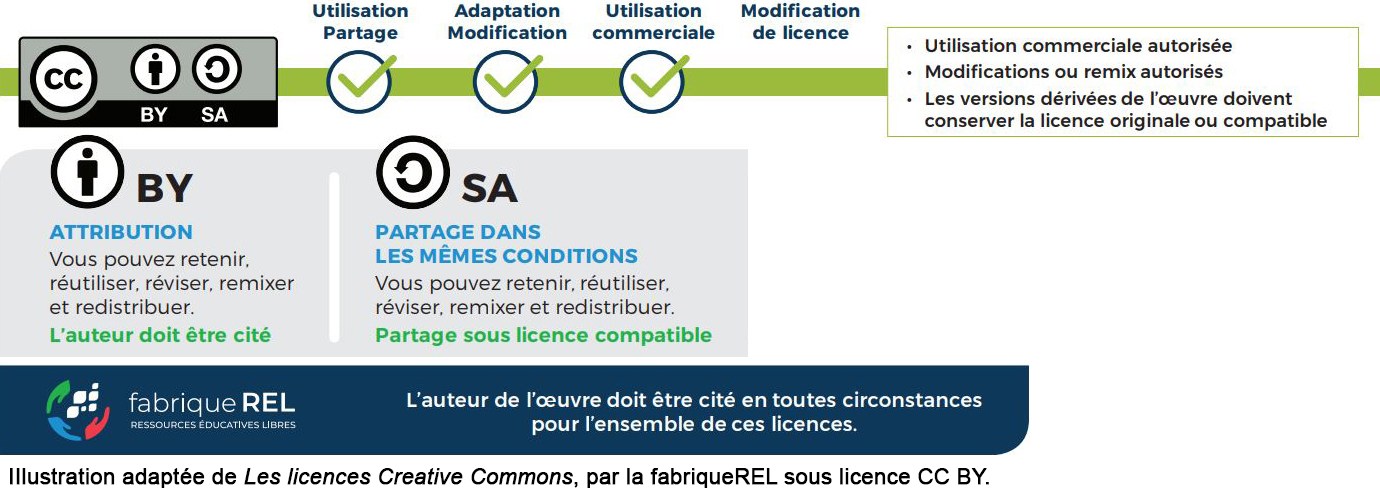
\includegraphics[width=0.8\textwidth,height=\textheight]{images/introduction/Licence.JPG}
\caption{Licence Creative Commons du livre}\label{fig-Licence}
}
\end{figure}

\textbf{Suggestions d'adaptation du manuel}

Pour chaque méthode de traitement d'image abordée dans le livre, une
description détaillée et une mise en œuvre dans Python sont disponibles.
Par conséquent, plusieurs adaptations du manuel sont possibles~:

\begin{itemize}
\item
  Conserver uniquement les chapitres sur les méthodes ciblées dans votre
  cours.
\item
  En faire une version imprimée et la distribuer aux personnes
  étudiantes.
\item
  Modifier la description d'une ou de plusieurs méthodes en effectuant
  les mises à jour directement dans les chapitres.
\item
  Insérer ses propres jeux de données dans les sections intitulées
  \emph{Mise en œuvre dans Python}.
\item
  Modifier les tableaux et figures.
\item
  Ajouter une série d'exercices.
\item
  Modifier les quiz de révision.
\item
  Rédiger un nouveau chapitre.
\item
  Modifier des syntaxes en Python. Plusieurs \emph{librairies} Python
  peuvent être utilisées pour mettre en œuvre telle ou telle méthode.
  Ces derniers évoluent aussi très vite et de nouvelles
  \emph{librairies} sont proposées fréquemment! Par conséquent, il peut
  être judicieux de modifier une syntaxe Python du livre en fonction de
  ses habitudes de programmation en Python (utilisation d'autres
  \emph{librairies} que ceux utilisés dans le manuel par exemple) ou de
  bien mettre à jour une syntaxe à la suite de la parution d'une
  nouvelle \emph{librairie} plus performante ou intéressante.
\item
  Toute autre adaptation qui permet de répondre au mieux à un besoin
  pédagogique.
\end{itemize}

\hypertarget{sect002}{%
\subsection*{Comment lire ce manuel?}\label{sect002}}
\addcontentsline{toc}{subsection}{Comment lire ce manuel?}

Le livre comprend plusieurs types de blocs de texte qui en facilitent la
lecture.

\textbf{Bloc \emph{packages}}

Habituellement localisé au début d'un chapitre, il comprend la liste des
\emph{packages} Python utilisés pour un chapitre.

\textbf{Bloc objectif}

Il comprend une description des objectifs d'un chapitre ou d'une
section.

\textbf{Bloc notes}

Il comprend une information secondaire sur une notion, une idée abordée
dans une section.

\textbf{Bloc pour aller plus loin}

Il comprend des références ou des extensions d'une méthode abordée dans
une section.

\textbf{Bloc astuce}

Il décrit un élément qui vous facilitera la vie~: une propriété
statistique, un \emph{package}, une fonction, une syntaxe Python.

\textbf{Bloc attention}

Il comprend une notion ou un élément important à bien maîtriser.

\textbf{Bloc exercice}

Il comprend un court exercice de révision à la fin de chaque chapitre.

\hypertarget{sect003}{%
\subsection*{Comment utiliser les données du livre pour reproduire les
exemples?}\label{sect003}}
\addcontentsline{toc}{subsection}{Comment utiliser les données du livre
pour reproduire les exemples?}

Ce livre comprend des exemples détaillés et appliqués en Python pour
chacune des méthodes abordées. Ces exemples se basent sur des jeux de
données ouverts et mis à disposition avec le livre. Ils sont disponibles
sur le \emph{repo github} dans le sous-dossier \texttt{data}, à
l'adresse
\url{https://github.com/serie-tele-pyton/TraitementImagesVol1/tree/main/data}.

Une autre option est de télécharger le \emph{repo} complet du livre
directement sur \emph{github}
(\url{https://github.com/serie-tele-pyton/TraitementImagesVol1}) en
cliquant sur le bouton \texttt{Code}, puis le bouton
\texttt{Download\ ZIP} (@fig-downloaffromgit). Les données se trouvent
alors dans le sous-dossier nommé \texttt{data}.

\begin{figure}
\hypertarget{fig-downloaffromgit}{%
\centering
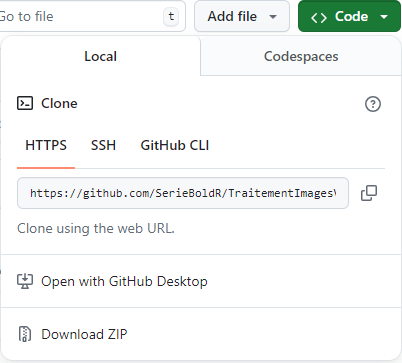
\includegraphics[width=0.4\textwidth,height=\textheight]{images/introduction/download_github.png}
\caption{Téléchargement de l'intégralité du
livre}\label{fig-downloaffromgit}
}
\end{figure}

\hypertarget{sect004}{%
\subsection*{Structure du livre}\label{sect004}}
\addcontentsline{toc}{subsection}{Structure du livre}

Le livre est organisé autour de quatre grandes parties.

\textbf{Partie 1. Importation et manipulation de données spatiales.}
Dans cette première partie, nous voyons comment importer, manipuler,
visualiser et exporter des données spatiales de type image (ou de type
matriciel) avec Python, principalement avec les \emph{packages}
\texttt{rasterio}, \texttt{xarray} et \texttt{numpy} ({[}chapitre
@sec-chap01{]}). Ce chapitre vous permettra de maîtriser la manipulation
à bas niveau de différents types d'imagerie. Différents exemples et
exercises sont disponibles avec différents capteurs satellites
(multi-spectral, RGB-NIR, SAR, etc.)

\textbf{Partie 2. Transformations des données spatiales}. Cette deuxième
partie comprend deux chapitres~: les transformations spectrales
({[}chapitre @sec-chap03{]}) et les transformations spatiales
({[}chapitre @sec-chap04{]}).

\textbf{Partie 3. Classifications d'images} Cette troisième partie
comprend deux chapitres~: les classifications supervisées ({[}chapitre
@sec-chap05{]}) et non supervisées ({[}chapitre @sec-chap06{]}).

\textbf{Partie 4. Données massives}. Cette quatrième et dernière partie
comprend un seul chapitre qui est dédié aux plateformes de mégadonnes
{[}chapitre @sec-chap07{]}, notammment Google Earth Engine.

\hypertarget{sect005}{%
\subsection*{Remerciements}\label{sect005}}
\addcontentsline{toc}{subsection}{Remerciements}

De nombreuses personnes ont contribué à l'élaboration de ce manuel.

Ce projet a bénéficié du soutien pédagogique et financier de la
\href{https://fabriquerel.org/}{\textbf{\emph{fabriqueREL}}} (ressources
éducatives libres). Les différentes rencontres avec le comité de suivi
nous ont permis de comprendre l'univers des ressources éducatives libres
(REL) et notamment leurs \href{https://fabriquerel.org/rel/}{fameux 5R}
(Retenir --- Réutiliser --- Réviser --- Remixer --- Redistribuer), de
mieux définir le besoin pédagogique visé par ce manuel, d'identifier des
ressources pédagogiques et des outils pertinents pour son élaboration.
Ainsi, nous remercions chaleureusement les membres de la
\emph{fabriqueREL} pour leur soutien inconditionnel~:

\begin{itemize}
\item
  Myriam Beaudet, bibliothécaire à l'Université de Sherbrooke.
\item
  Marianne Dubé, coordonnatrice de la fabriqueREL, Université de
  Sherbrooke.
\item
  Serge Piché, conseiller pédagogique, Université de Sherbrooke.
\item
  Claude Potvin, conseiller en formation, Service de soutien à
  l'enseignement, Université Laval.
\end{itemize}

Nous remercions chaleureusement les personnes étudiantes des cours
\textbf{à modifier plus tard} du
\href{https://www.usherbrooke.ca/admission/programme/271/baccalaureat-en-geomatiqueappliquee-a-lenvironnement/}{Baccalauréat
en géomatique appliquée à l'environnement} et du
\href{https://www.usherbrooke.ca/admission/programme/429/microprogramme-de-1er-cycleen-geomatique-appliquee/}{Microprogramme
de 1er cycle en géomatique appliquée} du
\href{https://www.usherbrooke.ca/geomatique/}{Département de géomatique
appliquée} de l'\href{https://www.usherbrooke.ca/}{Université de
Sherbrooke} de la session d'été 2023~: à modifier plus tard.

Nous remercions aussi les membres du comité de révision pour leurs
commentaires et suggestions très constructifs. Ce comité est composé de
quatre personnes étudiantes du
\href{https://www.usherbrooke.ca/geomatique/}{Département de géomatique
appliquée} de l'\href{https://www.usherbrooke.ca/}{Université de
Sherbrooke}~:

\begin{itemize}
\item
  À compléter plus tard.
\item
  À compléter plus tard.
\end{itemize}

Finalement, nous remercions Denise Latreille, réviseure linguistique et
chargée de cours à l'Université Sherbrooke, pour la révision du manuel.

\hypertarget{sect006}{%
\subsection*{Introduction aux images de télédétection}\label{sect006}}
\addcontentsline{toc}{subsection}{Introduction aux images de
télédétection}

L'imagerie numérique a pris une place importante dans notre vie de tous
les jours depuis une quinzaine d'année. Ces images sont prises
généralement au niveau du sol (imagerie proximale) avec seulement trois
couleurs dans le domaine de la vision humaine (rouge, vert et bleu).
Dans la suite du manuel, on parlera d'images du domaine de la vision par
ordinateur ou images en vision pour faire plus court.

Les images de télédétection ont des particularités et des propriétés qui
les différencient des images de tous les jours. On peut souligner au
moins cinq caractéristiques principales:

\begin{enumerate}
\def\labelenumi{\arabic{enumi}.}
\item
  Les images sont géoréférencées : Cela veut dire que pour chaque pixel
  nous pouvons y associer une position géographique ou cartographique.
\item
  Le point de vue est très différent : Ces images sont prises avec une
  vue d'en haut (Nadir) ou oblique avec une distance qui peut être très
  grande (On parle d'images distales).
\item
  Elles possèdent plus que 3 bandes : Contrairement aux images en
  vision, les images de télédétection possèdent bien souvent plus que 3
  bandes. Il n'est pas rare de trouver 4 bandes (Pléiade), 13 bandes
  (Sentinel-2, Landsat) et même 200 bandes pour des capteurs
  hyperspectraux.
\item
  Elles peuvent être calibrées : Les valeurs numérique de l'image
  peuvent être converties en quantités physiques (luminance,
  réflectance, section efficace, etc.) via une fonction de calibration.
\item
  Elles sont de grande taille : Il n'est pas rare de manipuler des
  images qui font plusieurs dizaines de milliers de pixels en dimension.
\end{enumerate}

\hypertarget{ressources-en-ligne}{%
\subsubsection{Ressources en ligne}\label{ressources-en-ligne}}

\hypertarget{sect0071}{%
\subsubsection*{\texorpdfstring{Listes des \emph{librairies}
utilisés}{Listes des librairies utilisés}}\label{sect0071}}
\addcontentsline{toc}{subsubsection}{Listes des \emph{librairies}
utilisés}

Dans ce livre, nous utilisons de nombreux \emph{packages} Python que
vous pouvez installer en une seule fois (voir {[}section @sec-00-01{]})
ou chapitre par chapitre.


    % Add a bibliography block to the postdoc
    
    
    
\end{document}
